% !TEX program = xelatex

\documentclass[aspectratio=169]{beamer}
% Template: https://www.overleaf.com/latex/templates/pure-minimalistic-a-truly-minimalistic-and-configurable-beamer-theme/hbvwphdxcbhf
%%%% Theme settings %%%%
\usepackage[utf8]{inputenc}
\usepackage[T1]{fontenc}
\usepackage{tikz}
\usetheme[nofooterlogo, showmaxslides, darkmode]{pureminimalistic}

% Logos
\renewcommand{\logotitle}{\includegraphics%
  [width=.6\linewidth]{logos/NAF_Logo.png}}
\renewcommand{\logoheader}{\includegraphics%
  [width=.8\linewidth]{logos/NAF_Logo.png}}
\renewcommand{\logofooter}{}

% Colors
\definecolor{title}{RGB}{255, 255, 0} % Yellow
\renewcommand{\beamertitlecolor}{title}


\usepackage{listings}
\usepackage{minted}


\title[How my first Network Automation project failed (and is still in production)]{How my first Network Automation project failed \\ (and is still in production)}
\author{Urs Baumann}
\institute{Swisscom}
\date{29.05.2024}

\begin{document}


{
% set background image for first page
\setbeamertemplate{background}
{
  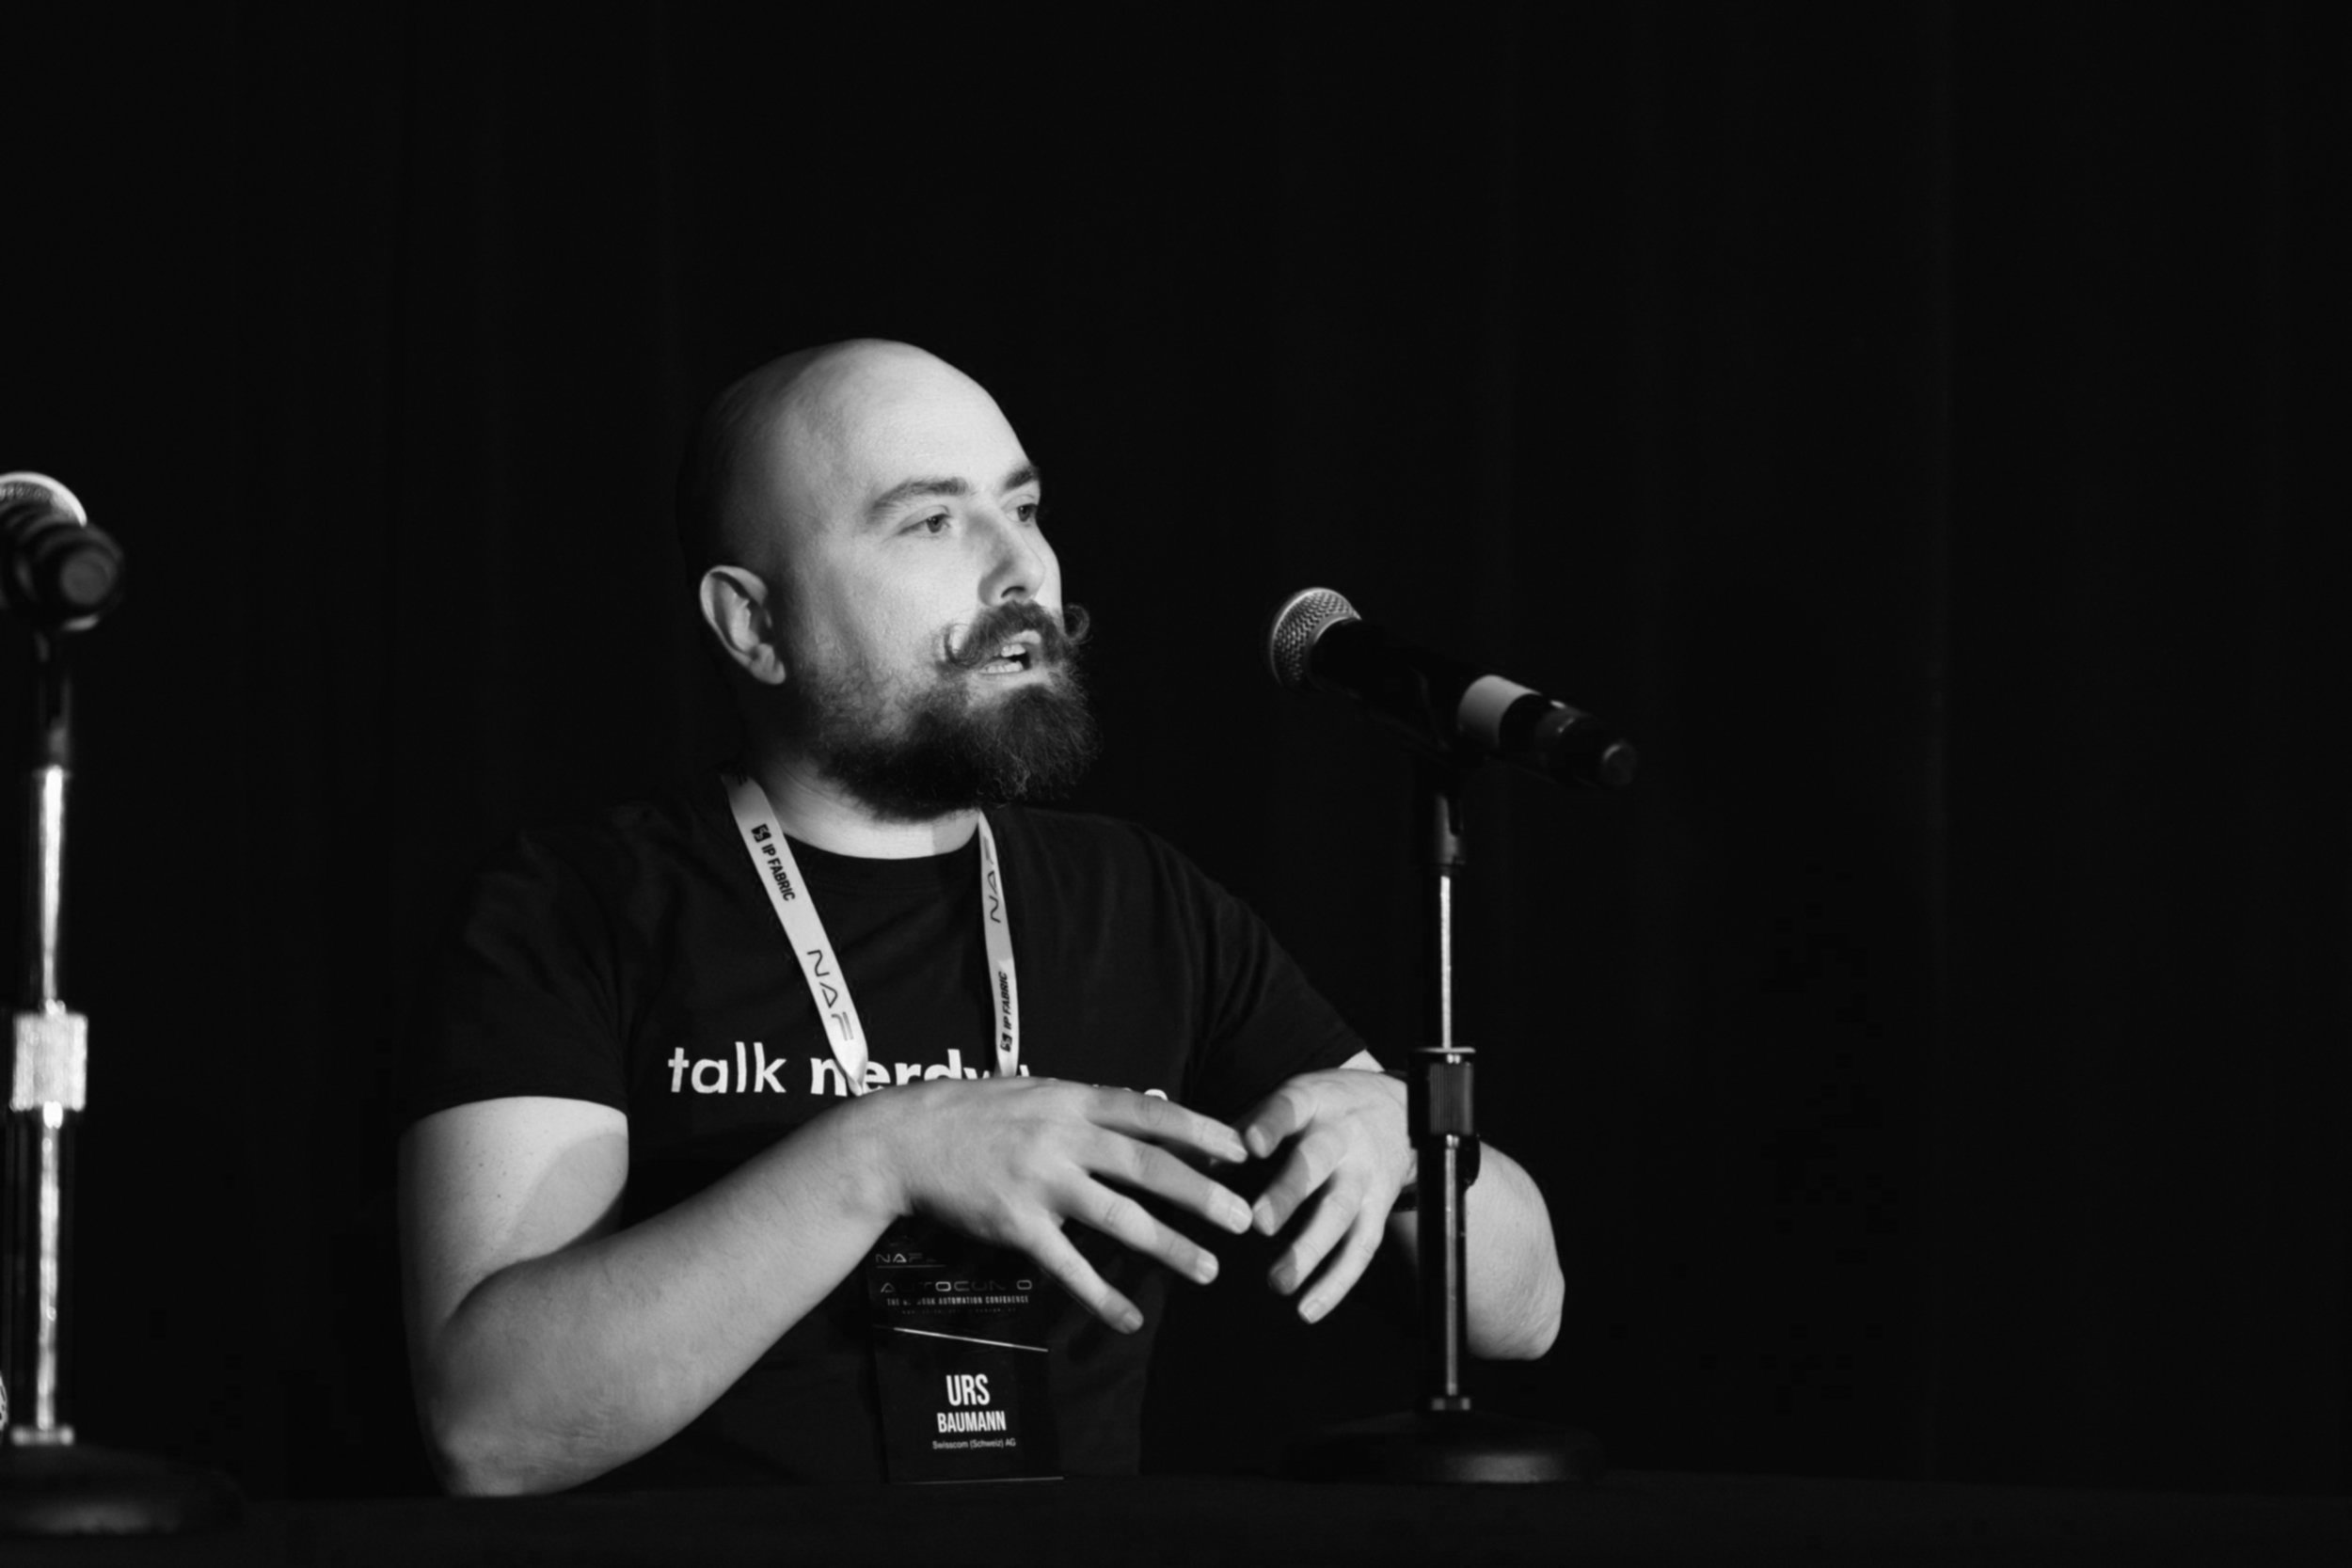
\includegraphics[height=\paperheight]{images/AutoCon_0-108.jpg}
}
\frame{\titlepage}
}

% \begin{frame}
%   \frametitle{Urs Baumann}
%   This is some text in the first frame. This is some text in the first frame. This is some text in the first frame.
% \end{frame}


\begin{frame}[fragile]
  \frametitle{Urs Baumann}

  \begin{minted}[fontsize=\small]{python}
>>> qr = QRCode()
>>> qr.add_data("https://www.linkedin.com/in/ubaumannch")
>>> qr.print_ascii()
  \end{minted}
  \begin{minted}[fontsize=\tiny]{text}
      █▀▀▀▀▀█ ▄ █▄▄ ▀█ ▀██▄ █▀▀▀▀▀█
      █ ███ █  ▀▄██ ▄▀  ▄█▀ █ ███ █
      █ ▀▀▀ █ ▀▀▄ ▄█▀█ ███  █ ▀▀▀ █
      ▀▀▀▀▀▀▀ ▀ █▄▀▄▀ █▄█ █ ▀▀▀▀▀▀▀
      ▀ █▄▀▄▀  █▀ ▀▀▀▀█▀▀▀▀▄▄ ▀▄ ▀▄
      ▄▀▀▄ ▄▀███▄█▄█▄▄ █▄ ██  ▄ ▀█▀
      ▀█▄▄▄ ▀▄ ▄█▄▀ ▀ █▀ ▀███▄ █ ▀█
      ▄██ █ ▀█ ▄▄▀▀▀ ▄▄▄█▄   ▀ █ █▀
      ▀▀█▄▀ ▀▀   ▄█▄ ▀█▀ ▀███▀ █▄▀█
      ▀▄▄█▄▀▀ ▀▄   ▄█▄▄█ ▄██▄▀ ▄ █▀
      ▀  ▀ ▀▀ █▄██  █ ▄▀▀▄█▀▀▀█ ▄▄▄
      █▀▀▀▀▀█  ▄▀▄▀▀ ▄ █▄▀█ ▀ ██ ▀█
      █ ███ █ ▀██▀▀▄  ██▄ ▀▀▀▀█ ▄██
      █ ▀▀▀ █ ▀ ▄▄█ █ ▀▄▄██▄▄▀█▀ ▄▀
      ▀▀▀▀▀▀▀ ▀▀ ▀▀▀▀ ▀▀ ▀▀▀ ▀▀▀ ▀▀
  \end{minted}
\end{frame}


% \begin{frame}[fragile]
%   \begin{columns}
%     \begin{column}{0.3\textwidth}
%       \begin{minted}{yaml}
% name: sw01
% domain_name: lab.ins
% syslog: 10.10.0.11
% interfaces:
% - Loopback0
% - Mgmt0/0
% - GigabitEthernet1/0/1
% bgp:
% asn: 65000
% \end{minted}
%     \end{column}
%     \begin{column}{0.3\textwidth}

%       \begin{minted}{django}
% !
% ! version 17
% !
% hostname {{ name }}
% ip domain name {{ domain_name }}
% logging server {{ syslog }}
% !
% 
% interface {{ nic }}
% no shutdown
% !
% 
% !
% 
% router bgp {{ bgp.asn }}
% 
% \end{minted}
%     \end{column}
%   \end{columns}
% \end{frame}


\end{document}